%% Documentclass:
%% Network Neuroscience
%\documentclass[finalfonts,NETN]{stjour}
\documentclass[NETN]{stjour}

%% or 

%% Manuscript, for double spaced, larger fonts
%\documentclass[manuscript]{stjour}
%% Only needed if you use `manuscript' option
% \journalname{Network Neuroscience}


%%%%%%%%%%% Article Set-Up %%%%%%%%%%%%%%%%%%%%%%%%%%%%%%%%%%%%
%% Article Type:
%% Default is Research.

%% Or, choose one of these options:
%% Research, Methods, Data, Review, and Perspective

\articletype{Research Article}

%%%%%%%%%%% Please supply information %%%%%%%%%%%%%%%%%%%%%%%%%

\supportinginfo{dx.doi.org/10.7910/DVN/PQ6ILM}

%% if no conflicts, this command doesn't need to be used
%% \conflictsofinterest{}

%%%%%%%%%%% to be supplied by MIT Press, only %%%%%%%%%%%%%%%%%
\citation{Betzel, R. F., Fukushima, M.,
He, Ye,
Zuo, Xi-Nian,
Sporns, O. (2016)\\
Dynamic fluctuations coincide with periods of high and low modularity
in resting-state functional brain  networks\\
Network Neuroscience, 1
}

\received{20 October 2016}
\accepted{7 November 2016}
\published{26 January 2016}
\setdoi{10.1162/NETN-00001} %% ???

\handlingeditor{Xi-Nian Zuo}

%%%%%%%% End MIT Press commands %%%%%%%%%%

%%%%%%%%%%%%%%%%%%%%%%%%%%%%%%%%%%%%%%%%%%%%%%%%%%%%%%%%%%%%%%%
%% author definitions should be placed here:

%% example definition
\def\taupav{\tau_{\mathrm{Pav}}}

\begin{document}
\title[Co-citations in context]{Co-citations in context}
\subtitle{Disciplinary heterogeneity is relevant}

%% If shortened title for running head is needed so that the article title can fit
%%   in the running head, use [] argument, ie,
%%
%%   \title[Shortened Title for Running Head]{Title of Article}
%%   \subtitle{Subtitle Here}

%% Since we use \affil{} in the argument of the \author command, we
%% need to supply another version of the author names, without \affil{}
%% to be used for running heads:

\author[Author Names]
{James Bradley\affil{1},
Sitaram Devarakonda\affil{2}, Avon Davey\affil{2}, Dmitriy Korobskiy\affil{2}, Siyu Liu\affil{2}, Tandy Warnow\affil{3}
\and George Chacko\affil{2}}

\affiliation{1}{Raymond A. Mason School of Business, College of William and Mary, Williamsburg, VA, USA}
\affiliation{2}{Netelabs, NET ESolutions Corporation, McLean, VA 22102, USA}
\affiliation{3}{Department of Computer Science, University of Illinois Urbana-Champaign, Champaign, IL 61820, USA}


%ie.
%\affiliation{1}{Gatsby Computational Neuroscience Unit, University
%College London, London, United Kingdom} 

%\affiliation{2}{Another Department, Institution, City, Country}

%ie
%\affiliation{2}{Center for Studies in
%Behavioral Neurobiology, Concordia University, Montreal, Quebec,
%Canada}

\correspondingauthor{George Chacko}{netelabs@nete.com}

% ie,
%\correspondingauthor{Ritwik K. Niyogi}{ritwik.niyogi@gatsby.ucl.ac.uk}

\keywords{(bibliometrics, co-citation analysis, random graphs )}

%ie
%\keywords{work, leisure, normative, microscopic,  reinforcement learning, economics}

\begin{abstract}
Citation analysis of the scientific literature has been used to study and define disciplinary boundaries, to trace the dissemination of knowledge, and to estimate impact. Co-citation, the frequency with which pairs of publications are cited, provides insight into how documents relate to each other and across fields. Co-citation analysis has been used to characterize combinations of prior work as conventional or innovative and to derive features of highly cited publications. Given the organization of science into disciplines, a key question is the sensitivity of such analyses to frame of reference. Our study examines this question using  semantically-themed citation networks. We observe that trends reported to be true across the scientific literature do not hold for focused citation networks, and conclude that co-citation analysis requires a contextual perspective.
\end{abstract}

% \begin{authorsummary} 
% \end{authorsummary}


\section{Introduction}
Citation and network analysis of  scientific literature reveals information on semantic relationships between publications, collaboration between scientists, and the practice of citation itself~\cite{de_solla_price_networks_1965,newman_structure_2001}. Co-citation, the frequency with which two documents are cited together in other documents~\cite{small_co-citation_1973,marshakova-shaikevich_co-citation_1973}, provides additional insights, including the identification of semantically related documents and fields. Uzzi et al. applied co-citation analysis to 17.9 million publications from the Web of Science (WoS) to identify novel combinations of prior research and to characterize highly cited papers. They analyzed co-citations of references (and journals) within publications, and computed a `z-score' for each journal pair using Monte Carlo simulations based on a random graph model. The set of journal-pair z-scores for each publication was  used to assess  conventionality and novelty, resulting in four categories: high or low conventionality (HC or LC) and high or low novelty (HN or LN), and all four combinations are possible. The authors concluded that highly cited publications across the research literature (and within most subfields) are more likely to be characterized as HC and HN than less highly cited publications.  Key to Uzzi is their random graph model, where  a reference cited in a publication is randomly replaced by another article from the same year as the cited reference, thus producing a random assignment of references to each paper. The model treats potential substitutions as equi-probable, irrespective of disciplinary origin. Accordingly, we hypothesize that analyzing semantically related sets of documents (and limiting substitutions to the citations in the local network) will reduce model misspecification and better simulate citation practice, leading to different and more relevant conclusions.  
We developed a highly efficient algorithm to simulate under a refined random graph model. Our study on three semantically-themed citation networks reveals significantly different patterns of conventionality and novelty between  citation networks and disciplines.

\subsection{Sample Subsection}
Text here. Text here. Text here. Text here.
Text here. Text here. Text here. Text here.
Text here. Text here. Text here. Text here.
Text here. Text here. Text here. Text here.

\subsubsection{Sample Subsubsection}
Text here. Text here. Text here. Text here.
Text here. Text here. Text here. Text here.
Text here. Text here. Text here. Text here.
Text here. Text here. Text here. Text here.


\section{Sample equations}
\begin{equation}
\label{eq:rhoCHT}
\rho^{\pi}= \frac{RI + \mathbb{E}_{\pi([L,\tau_L]|\textrm{post})}
\left[C_L(\taupav+\tau_L) \right]   +
\displaystyle{\int_{0}^{P}}{dw~ \mathbb{E}_{\pi_{w_L}}}
\Biggl[\/\sum_{n_{L|[\textrm{pre},w]}}C_L(\tau_L)
\Biggr]            }      {P +
\mathbb{E}_{\pi([L,\tau_L] |\textrm{post})}[\tau_{L}] +\taupav +
\displaystyle{ \int_{0}^{P}}{dw~ \mathbb{E}_{\pi_{w_L}}}   
\Biggl[\sum_{n_{L|[\textrm{pre},w]}}\tau_L\Biggr]  
}
\end{equation}
As long as
$RI - K_LP > 
\frac{1}{\beta}$
\begin{equation}
%\def\theequation{5.1}
\left.\begin{array}{lrcl}
&\rho^{\pi} &=&  \displaystyle\frac{\beta ( RI + K_L \taupav )-1} {\beta
(P+\taupav )}    \\[12pt]
\hbox{and}\hbox to .25in{\hfill}&\mathbb{E}[\tau_L | \text{post}] &=&\displaystyle \frac{P+\taupav}{\beta ( RI -
K_LP)-1}  
\label{eq:analytical_linear}
\end{array}\right\}\hbox to 1.25in{\hfill}
\end{equation} 
Text finishing first page.
Text finishing first page.
Text finishing first page.
Text finishing first page.
Text finishing first page.
Text finishing first page.
Text finishing first page.


\begin{boxedtext}{Comparative Analysis of Different Classes of Networks} 
Going beyond the examination of shared topological features across
nervous systems, the generalized mathematical language of graph theory
also offers tools for the comparison of the organization of brain
networks to other classes of network studied
by different scientific
disciplines. 

Many real-world systems operate as some sort of
interaction or communication network, including, for example, social
networks, gene regulatory networks, computer networks, and
transportation networks. Similar to brain networks, many of these
real-world networks display an efficient small-world organization, a
pronounced community structure with densely connected modules, as well
as the formation of hubs and rich clubs. Going beyond the
comparison of networks within the class of nervous systems, the field
of `comparative network analysis' examines commonalities and
differences across a range of network classes.

\begin{figure}
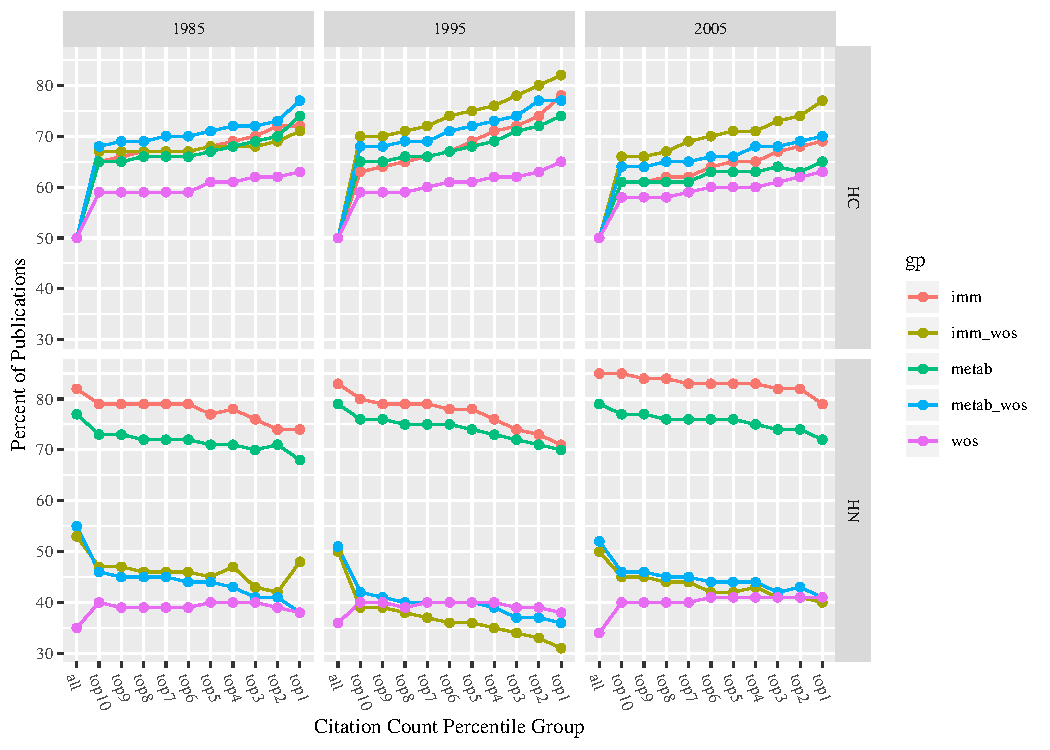
\includegraphics[width=\hsize]{Fig1}
\caption{Here is the caption.}
\end{figure}
\end{boxedtext}

\newpage
\begin{boxedtext}{Comparative Analysis of Different Classes of Networks} 
Going beyond the examination of shared topological features across
nervous systems, the generalized mathematical language of graph theory
also offers tools for the comparison of the organization of brain
networks to other classes of network studied by different scientific
disciplines. Many real-world systems operate as some sort of
interaction or communication network, including, for example, social
networks, gene regulatory networks, computer networks, and
transportation networks. Similar to brain networks, many of these
real-world networks display an efficient small-world organization, a
pronounced community structure with densely connected modules, as well
as the formation of hubs and rich clubs. Going beyond the
comparison of networks within the class of nervous systems, the field
of `comparative network analysis' examines commonalities and
differences across a range of network classes.

\begin{table}[ht]
\caption{Here is the caption.}

\centerline{\begin{tabular}{|c|c|c|}
\hline
one&two&three\\
\hline
four&five&six\\
\hline
\end{tabular}}
\end{table}
\end{boxedtext}

\subsection{Jargon Samples in margin}
One common decision is between working (performing an employer-defined
task) and engaging in leisure (activities pursued for oneself). Working
leads to external rewards such as food and money; whereas leisure is
supposed to be intrinsically beneficial \jargon{Intrinsically beneficial}{The characteristic of
leisure that we enjoy most.} (otherwise one would not want to
engage in it).
%% \jargon has optional argument in square brackets where you can specify
%% the amount of extra space below where it would normally appear when 
%% two \jargon entries are in the same paragraph:
$\beta \in [0,\infty)$\jargon[24pt]{$\beta \in [0,\infty)$}{inverse temperature or degree of
stochasticity-determinism parameter.} is often used to indicate an
important parameter, the stochasticity-determinism parameter.

\subsection{Simple code sample}

\begin{code}
\begin{verbatim}
procedure bubbleSort( A : list of sortable items )
    n = length(A)
    repeat
       newn = 0
       for i = 1 to n-1 inclusive do
          if A[i-1] > A[i] then
             swap(A[i-1], A[i])
             newn = i
          end if
       end for
       n = newn
    until n = 0
end procedure
\end{verbatim}
\end{code}


\subsection{Algorithm environment}
%% \begin{algorithm} takes option [p][b][t][h],  or some combination, like \begin{figure}
%% See documentation for algorithmic.sty for more information on formatting algorithms.

\begin{algorithm}[h]
\caption{A sample in an algorithm environment.}
\begin{algorithmic}
\If {$i\geq maxval$}
    \State $i\gets 0$
\Else
    \If {$i+k\leq maxval$}
        \State $i\gets i+k$
    \EndIf
\EndIf
\end{algorithmic}
\end{algorithm}


\section{Itemized Lists}

\subsection{Roman list:}

\begin{enumerate}
\item[(i)] at high 
payoffs, subjects work almost continuously.
\item[(ii)] at low payoffs, they 
engage in leisure all at once, in long bouts after working.
\item[(iii)] subjects work continuously for the entire price duration, as long as
the price is not very long;
\item[(iv)] the duration of leisure bouts is variable.
\end{enumerate}


\subsection{Numbered list:}

\begin{enumerate}
\item at high 
payoffs, subjects work almost continuously, engaging in little leisure
inbetween work bouts; 
\item at low payoffs, they 
engage in leisure all at once, in long bouts after working, rather
than distributing the same amount of leisure time into multiple short
leisure bouts; 
\item subjects work continuously for the entire price duration, as long as
the price is not very long (as shown by an analysis conducted by
Y-AB, to be published separately);  
\item the duration of leisure bouts is variable.
\end{enumerate}


\subsection{Bulleted list:}

\begin{itemize}
\item at high 
payoffs, subjects work almost continuously, engaging in little leisure
inbetween work bouts; 
\item at low payoffs, they 
engage in leisure all at once, in long bouts after working, rather
than distributing the same amount of leisure time into multiple short
leisure bouts; 
\item subjects work continuously for the entire price duration, as long as
the price is not very long (as shown by an analysis conducted by
Y-AB, to be published separately);  
\item the duration of leisure bouts is variable.
\end{itemize}

\subsection{Description list:}
\begin{description}
\item[High payoffs:] at high 
payoffs, subjects work almost continuously, engaging in little leisure
inbetween work bouts; 
\item[Low payoffs:] at low payoffs, they 
engage in leisure all at once, in long bouts after working, rather
than distributing the same amount of leisure time into multiple short
leisure bouts; 
\item[Continuous work:] subjects work continuously for the entire price duration, as long as
the price is not very long (as shown by an analysis conducted by Y-AB, to be published separately); 
\item[Duration:] the duration of leisure bouts is variable.
\end{description}

\newpage
\section{Sample citations}
For general information on the correct form for citations using
the APA 6 format, see the following sites:
\href{https://owl.english.purdue.edu/owl/resource/560/02/}
{APA 6, In-text citations, The Basics} and
\href{https://owl.english.purdue.edu/owl/resource/560/03/}
{APA 6, In-text citations}



\section{Natbib citation mark up}

\subsection{Single citations}
\noindent
\begin{tabular}{ll}
\bf Type&\bf Results\\
\hline
\verb+\citet{jon90}+&\dogray Jones et al. (1990)\\
\verb+\citet[chap. 2]{jon90}+&\dogray Jones et al. (1990, chap. 2)\\
    \verb+\citep{jon90}+	    &\dogray   	(Jones et al., 1990)\\
    \verb+\citep[chap. 2]{jon90}+ 	&\dogray    	(Jones et al., 1990, chap. 2)\\
    \verb+\citep[see][]{jon90}+ 	 &\dogray    	(see Jones et al., 1990)\\
    \verb+\citep[see][chap. 2]{jon90}+ 	&\dogray    	(see Jones et al., 1990, chap. 2)\\
    \verb+\citet*{jon90}+ 	    &\dogray    	Jones, Baker, and Williams (1990)\\
    \verb+\citep*{jon90}+	    & \dogray   	(Jones, Baker, and Williams,
    1990) \\
\end{tabular}

For example, some citations from the NETNbibsamp.bib database:




citet: \citet{bullmore2009complex}, citep: \citep{gomez2009analysis}, and
citep*: \citep*{de2012cortical}

\subsection{Multiple citations}
Multiple citations may be made by including more than one citation
key in the \verb+\cite+ command argument.

\noindent
\begin{tabular}{ll}
\bf Type&\bf Results\\
\hline
\verb+\citet{jon90,jam91}+&\dogray Jones et al. (1990); James et al. (1991)\\
\verb+\citep{jon90,jam91}+&\dogray (Jones et al., 1990; James et al. 1991)\\
\verb+\citep{jon90,jon91}+&\dogray (Jones et al., 1990, 1991)\\
\verb+\citep{jon90a,jon90b}+&\dogray (Jones et al., 1990a,b)\\
\end{tabular}

For example, multiple citations from the bibsamp.bib database:
citet: \citet{nooner2012nki,hutchison2013resting},
 citep:
\citep{tagliazucchi2012dynamic, de2012cortical}

As you see, the citations are automatically hyperlinked to their
reference in the bibliography.

\newpage

\section{Sample figures}

\begin{figure}[h] 
\centerline{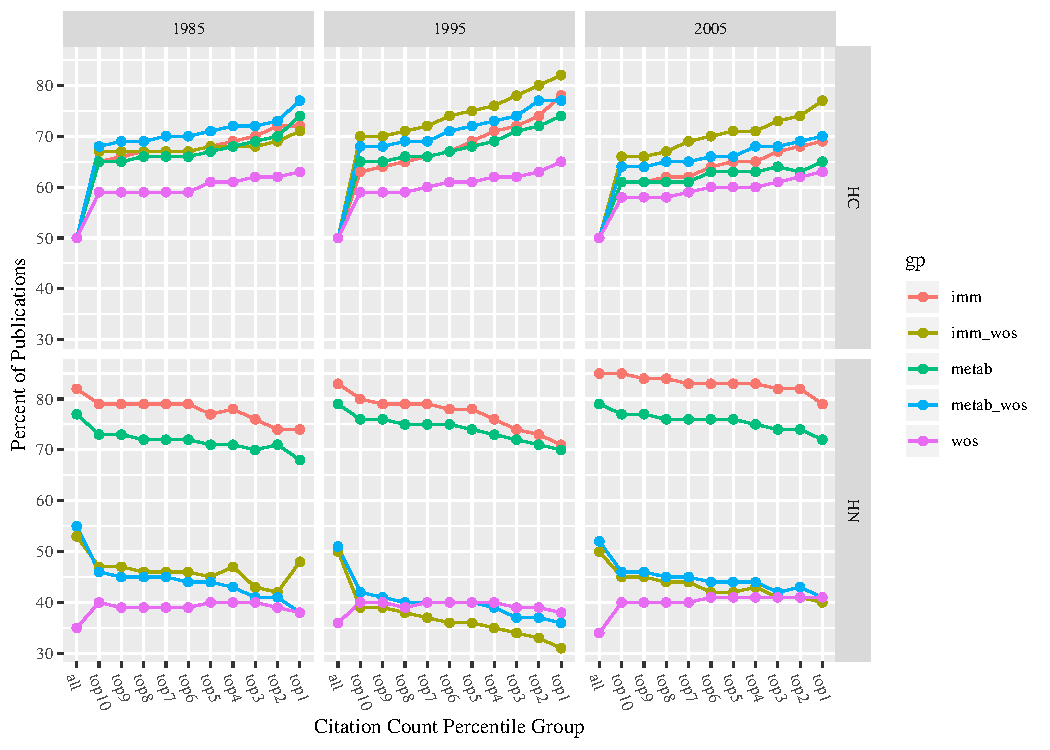
\includegraphics[width=\textwidth]{Fig1.pdf}}
\caption{(Colour online) \textbf{Task and key features of the
 data.} \\
 A) Cumulative handling time (CHT) task. Grey bars denote work
(depressing a lever), white gaps show leisure. The subject must
accumulate work up to a total period of time called the
\emph{price} ($P$) in order to obtain a single reward (black dot) of subjective reward
intensity $RI$. The trial duration is $25\times \mathrm{price}$ (plus
$2$s each time the price is attained, during which the lever is retracted so it cannot
work; not shown).}
\label{fig:task_data}
\end{figure}
%% this command ends a page but does not fill the bottom with white space:
\eject

\begin{figure}[ht] 
\widefigure{\fullpagewidth}{Fig1.pdf}
\caption{(Colour online) \textbf{Task and key features of the
 data.} \\
 A) Cumulative handling time (CHT) task. Grey bars denote work
(depressing a lever), white gaps show leisure. The subject must
accumulate work up to a total period of time called the
\emph{price} ($P$) in order to obtain a single reward (black dot) of subjective reward
intensity $RI$. The trial duration is $25\times \mathrm{price}$ (plus
$2$s each time the price is attained, during which the lever is retracted so it cannot
work; not shown).}
\label{fig:task_data2}
\end{figure}

\newpage
\section{Sample tables}

\begin{table}[!ht]
\caption{Time of the Transition Between Phase 1 and Phase 2$^{a}$}
\label{tab:label}
\centering
\begin{tabular}{lc}
\hline
 Run  & Time (min)  \\
\hline
  $l1$  & 260   \\
  $l2$  & 300   \\
  $l3$  & 340   \\
  $h1$  & 270   \\
  $h2$  & 250   \\
  $h3$  & 380   \\
  $r1$  & 370   \\
  $r2$  & 390   \\
\hline
\multicolumn{2}{l}{$^{a}$Table note text here.}
\end{tabular}
\end{table}

\begin{table}[ht]
\widecaption{Sample table taken from [treu03]\label{tbl-1}}
\begin{widetable}
\advance\tabcolsep-1pt
\small
\begin{tabular}{ccrrccccccccc}
\hline
\bf 
POS &\bf  chip &\multicolumn1c{\bf ID} &\multicolumn1c{\bf X}
&\multicolumn1c{\bf Y} &\bf
RA &\bf DEC &\bf IAU$\pm$ $\delta$ IAU &\bf
IAP1$\pm$ $\delta$ IAP1 &\bf IAP2 $\pm$ $\delta$
IAP2 &\bf star &\bf E &\bf Comment\\
\hline
0 & 2 & 1 & 1370.99 & 57.35\rlap{$^a$}    &   6.651120 &  17.131149 &
21.344$\pm$0.006\rlap{$^b$}  & 2 4.385$\pm$0.016 & 23.528$\pm$0.013 & 0.0 & 9 & -    \\
0 & 2 & 2 & 1476.62 & 8.03     &   6.651480 &  17.129572 & 21.641$\pm$0.005  & 2 3.141$\pm$0.007 & 22.007$\pm$0.004 & 0.0 & 9 & -    \\
0 & 2 & 3 & 1079.62 & 28.92    &   6.652430 &  17.135000 & 23.953$\pm$0.030  & 2 4.890$\pm$0.023 & 24.240$\pm$0.023 & 0.0 & - & -    \\
0 & 2 & 4 & 114.58  & 21.22    &   6.655560 &  17.148020 & 23.801$\pm$0.025  & 2 5.039$\pm$0.026 & 24.112$\pm$0.021 & 0.0 & - & -    \\
0 & 2 & 5 & 46.78   & 19.46    &   6.655800 &  17.148932 & 23.012$\pm$0.012  & 2 3.924$\pm$0.012 & 23.282$\pm$0.011 & 0.0 & - & -    \\
0 & 2 & 6 & 1441.84 & 16.16    &   6.651480 &  17.130072 & 24.393$\pm$0.045  & 2 6.099$\pm$0.062 & 25.119$\pm$0.049 & 0.0 & - & -    \\
0 & 2 & 7 & 205.43  & 3.96     &   6.655520 &  17.146742 & 24.424$\pm$0.032  & 2 5.028$\pm$0.025 & 24.597$\pm$0.027 & 0.0 & - & -    \\
0 & 2 & 8 & 1321.63 & 9.76     &   6.651950 &  17.131672 &
22.189$\pm$0.011  & 2 4.743$\pm$0.021 & 23.298$\pm$0.011 & 0.0 & 4 &
edge \\
\hline\\[-6pt]
\multicolumn{13}{l}{%
Table 2 is published in its entirety in the electronic
edition of the {\it Astrophysical Journal}.}\\[3pt]
\multicolumn{13}{l}{%
$^a$ Sample footnote for table 2.}\\[3pt]
\multicolumn{13}{l}{%
$^b$ Another sample footnote for table 2.}
\end{tabular}
\end{widetable}
\end{table}

\begin{table}[p]
\rotatebox{90}{\vbox{\hsize=\textheight
\caption{Here is a caption for a table that is found in landscape
mode.}
\begin{tabular}{ccrrccccccccc}
\hline
\bf 
POS &\bf  chip &\multicolumn1c{\bf ID} &\multicolumn1c{\bf X}
&\multicolumn1c{\bf Y} &\bf
RA &\bf DEC &\bf IAU$\pm$ $\delta$ IAU &\bf
IAP1$\pm$ $\delta$ IAP1 &\bf IAP2 $\pm$ $\delta$
IAP2 &\bf star &\bf E &\bf Comment\\
\hline
0 & 2 & 1 & 1370.99 & 57.35\rlap{$^a$}    &   6.651120 &  17.131149 &
21.344$\pm$0.006\rlap{$^b$}  & 2 4.385$\pm$0.016 & 23.528$\pm$0.013 & 0.0 & 9 & -    \\
0 & 2 & 2 & 1476.62 & 8.03     &   6.651480 &  17.129572 & 21.641$\pm$0.005  & 2 3.141$\pm$0.007 & 22.007$\pm$0.004 & 0.0 & 9 & -    \\
0 & 2 & 3 & 1079.62 & 28.92    &   6.652430 &  17.135000 & 23.953$\pm$0.030  & 2 4.890$\pm$0.023 & 24.240$\pm$0.023 & 0.0 & - & -    \\
0 & 2 & 4 & 114.58  & 21.22    &   6.655560 &  17.148020 & 23.801$\pm$0.025  & 2 5.039$\pm$0.026 & 24.112$\pm$0.021 & 0.0 & - & -    \\
0 & 2 & 5 & 46.78   & 19.46    &   6.655800 &  17.148932 & 23.012$\pm$0.012  & 2 3.924$\pm$0.012 & 23.282$\pm$0.011 & 0.0 & - & -    \\
0 & 2 & 6 & 1441.84 & 16.16    &   6.651480 &  17.130072 & 24.393$\pm$0.045  & 2 6.099$\pm$0.062 & 25.119$\pm$0.049 & 0.0 & - & -    \\
0 & 2 & 7 & 205.43  & 3.96     &   6.655520 &  17.146742 & 24.424$\pm$0.032  & 2 5.028$\pm$0.025 & 24.597$\pm$0.027 & 0.0 & - & -    \\
0 & 2 & 8 & 1321.63 & 9.76     &   6.651950 &  17.131672 &
22.189$\pm$0.011  & 2 4.743$\pm$0.021 & 23.298$\pm$0.011 & 0.0 & 4 &
edge \\
\hline\\[-6pt]
\multicolumn{13}{l}{%
Table 2 is published in its entirety in the electronic
edition of the {\it Astrophysical Journal}.}\\[3pt]
\multicolumn{13}{l}{%
$^a$ Sample footnote for table 2.}\\[3pt]
\multicolumn{13}{l}{%
$^b$ Another sample footnote for table 2.}
\end{tabular}
}}
\end{table}
\clearpage
\begin{boxedtext}{Tools for comparison of networks} 
Going beyond the examination of shared topological features across
nervous systems, the generalized mathematical language of graph theory
also offers tools for the comparison of the organization of brain
networks to other classes of network studied by different scientific
disciplines. 

From $\mathcal{W}$, we can estimate the variability in the fluctuations of the functional connection between nodes $i$ and $j$ over time as:
\begin{equation}
s_{ij}=\sqrt{\frac{1}{T-L}\sum_{t=1}^{T-L+1}(W_{ij}(t) - m_{ij})}
\end{equation}
where $m_{ij}=\frac{1}{T-L+1}\sum_{t=1}^{T-L+1}W_{ij}(t)$ is the mean
dynamic functional connectivity over time. 

Many real-world systems operate as some sort of
interaction or communication network, including, for example, social
networks, gene regulatory networks, computer networks, and
transportation networks. Similar to brain networks, many of these
real-world networks display an efficient small-world organization, a
pronounced community structure with densely connected modules, as well
as the formation of hubs and rich clubs. Going beyond the
comparison of networks within the class of nervous systems, the field
of `comparative network analysis' examines commonalities and
differences across a range of network classes.
\end{boxedtext}

Example of table continuing over pages:


\begin{center}
\begin{longtable}{ccc@{}}
\caption{ApJ costs from 1991 to 2013
\label{tab:table}} \\[2pt]
\hline
\bf Year & \bf Subscription & \bf Publication \\
 & \bf cost &\bf charges\\
 & \bf(\$) & \bf (\$/page)\\
\hline
\endfirsthead

\multicolumn3c{Table \thetable, \it continued from previous page.}\\[6pt]
\multicolumn3c{ApJ costs from 1991 to 2013}\\[2pt]
\hline
\bf Year & \bf Subscription & \bf Publication \\
 & \bf cost &\bf charges\\
 & \bf(\$) & \bf (\$/page)\\
\hline
\endhead
\\\hline
\\[-8pt]
\multicolumn{3}{r}{\it Table continued on next page}\\ 
\endfoot

\hline
\endlastfoot

1991 & 600 & 100 \\
1992 & 650 & 105 \\
1993 & 550 & 103 \\
1994 & 450 & 110 \\
1995 & 410 & 112 \\
1996 & 400 & 114 \\
1997 & 525 & 115 \\
1998 & 590 & 116 \\
1999 & 575 & 115 \\
2000 & 450 & 103 \\
2001 & 490 &  90 \\
2002 & 500 &  88 \\
2003 & 450 &  90 \\
2004 & 460 &  88 \\
2005 & 440 &  79 \\
2006 & 350 &  77 \\
2007 & 325 &  70 \\
2008 & 320 &  65 \\
2009 & 190 &  68 \\
2010 & 280 &  70 \\
2011 & 275 &  68 \\
2012 & 150 &  56 \\
2013 & 140 &  55 \\
\end{longtable}
\end{center}

\section{Supportive Information}
Here you enter further sources of information, if desired.

%% A possible entry might be:
% No supportive information is available at this time.


\acknowledgments
Enter your acknowledgments here.

%% ie.,

% The authors thank Laurence Aitchison for fruitful discussions.  RKN
% and PD received funding from the Gatsby Charitable Foundation. Y-AB,
% RBS, KC and PS received funding from Canadian Institutes of Health
% Research grant $MOP74577$,
% Fond de recherche Qu\'{e}bec - Sant\'{e} (Group grant to the Groupe 
% de recherche en neurobiologie comportementale, Shimon Amir, P.I.), and
% Concordia University Research Chair (Tier I). 

\authorcontributions 
Who helped formulate the project, who supplied data, analyses and
experiments, etc.

%% ie.
%% Project was formulated by RKN, PD, PS,
%% based on substantial data, analyses and experiments of Y-AB, KC, RS,
%% PS. RKN, PD formalised the model, RKN implemented and ran the model;
%% RKN analysed the molecular ethogram data; Y-AB formalised and
%% implemented a CTMC model. All authors wrote the manuscript.




\section{Making Your Bibliography for a Network Neuroscience Article}
{\it Network Neuroscience} uses the APA author-date  bibliography style,
apacite.bst. For more
information on apacite, for examples in how to make your .bib file and more, see:\\
\href{http://mirror.jmu.edu/pub/CTAN/biblio/bibtex/contrib/apacite/apacite.pdf}
{http://mirror.jmu.edu/pub/CTAN/biblio/bibtex/contrib/apacite/apacite.pdf}

\noindent
(In spite of the mention of apacite cite commands, please use only
Natbib commands for in text citations, as shown above.)

\subsection{BibTeX}
You will need to use BibTeX to form your bibliography; typing in the
references would be
a huge and unpleasant task. Look at the NETNSample.bbl file and you'll see why
typing in the bibitems would be difficult. 

For a good basic introduction to using BibTeX, see\\
\href{https://www.economics.utoronto.ca/osborne/latex/BIBTEX.HTM}
{https://www.economics.utoronto.ca/osborne/latex/BIBTEX.HTM}

When you use BibTeX, the form of the bibliography will be correct. You
don't need to supply a bibliography style, since that is built into
the stjour.cls file when the NETN option is used
(\verb+\documentclass[NETN]{stjour}+).



\newpage
\subsection{Sample citations}

Here are some samples using \verb+\citep{}+:\\
\citep{bullmore2009complex,
gomez2009analysis,
rubinov2011weight,
power2014methods,
sporns2015modular,
scheeringa2012eeg,
fortunato2007resolution,
reichardt2006statistical,
smith2009correspondence,
sporns2011networks,
liegeois2014cerebral}

And more using \verb+\citet{}+\\
\citet{allen2012tracking,
calhoun2014chronnectome,
liu2013time,
fisher1915frequency,
gonzalez2014spatial,
damaraju2014dynamic,
hutchison2013resting,
de2012cortical,
tagliazucchi2012dynamic,
nooner2012nki}

\newpage
%%%%%%%%%%%%%%%%%%%%%%%
%% The bibliography

\bibliography{cocit_r}


%% No appendices allowed in Network Neuroscience style
%\appendix

\end{document}

